
\chapter*{Game Engines}
\addcontentsline{toc}{chapter}{Framework Maker for Games}
  \textbf{Building your own game engine is the standard practice when it comes to large in-house development teams.}
  This of course, comes with both advantages and disadvantages.
  The advantages are spaced around the ideas of security and integrity.
  While the disadvantages are mostly cost-related.

  Smaller companies often turn to open-source software as a solution. There are several providers in the market, such as Unity, Unreal, and Godot. Other notable names include P5.js, Processing, and even content creators like The Coding Train, Sebastian Lague, and Code Bullet, as well as electronics expert Ben Eater.

  If you're not familiar with these references, don't worry. The following sections will provide more in-depth insights into each of them.

  \section*{Overview}

  As I have already previously mentioned, this is a standardized practice that seems to return profit on investment.
  Large part of the returnment is based around security, bussines integrity and competitive edge.
  
  Not many of those closed-source software had ever seen the light of end-users' eyes. Some get leaked sometimes. (Figure:)


  On the other side of the spectrum live the restricted source software and the open sourse software.

  In the following i will like us to analyse some of the following game engine environments and draw out relevant particularities

% TODO TODO
% 1 Open Source graphics framework (p5.js), 1 closed software game engine (RAGE) and 1 restricted game engine (UNITY).

% TEXT::TEXT

% already existing reources and docs, community, 
%           disadvantages:  dificult to come up with unique style.


        %   \subsubsection*{RAGE}
        %       this is a closed, unaccesible project, 
        %       and we're looking at it..

        %   \subsubsection*{Unity}
        %       Unity's source code is not accesible to the public, the engine is completly free to use for any individual*.

        %   \subsubsection*{P5.js}
        %       This graphics engine is completly \textbf{\emph{free}}
        %       with \href[]{github.com}{source code}



\chapter*{Machine Learning}
\addcontentsline{toc}{chapter}{the pitch}
    \textbf{Machine Learning is a fun/handy technology to integrate.}

    is eye candy, everyone implements it into anything. Let's see how they did it.

    What other reasons could there be for wanting to implement it?

    \section*{Dialogue is important in simulators.}

      In game design, it's a known fact that the npcs are there to guide the player, are the pawns in a chess game. They are an immovable objects that determines the max speed of the unstoppable force.

      This static elements could be greatly improved. 
      \textbf{Not only gamers would benefit from dialogue improvements!}

        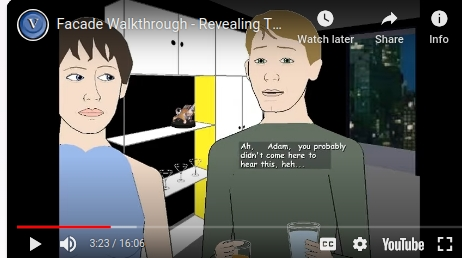
\includegraphics[width=0.8\textwidth]{facade.jpeg}

        NPCs are there to guide the player and are the projection of the game designers into the game world. 

        Because of this, is is really important that npcs have fluid dialogue and dont break the illusion of choice too easily.
        Current solutions imply using dialogue trees.
        Dialogue trees are an really good solution but they can still feel rough on the edges. and the illusion can be broken easily when u have to decide from a set of predefined dialogue choices.

        The imersiveness of games could greatly improve if ml were to be implemented on top of this already existing dialogue tree solution.

        Such solutions have already been experimented with, in the following i will present the findings of 2 other papers that use machine learning to improve npc dialogue and interaction.



        % \begin{figure}
        %   \begin{center}
        %     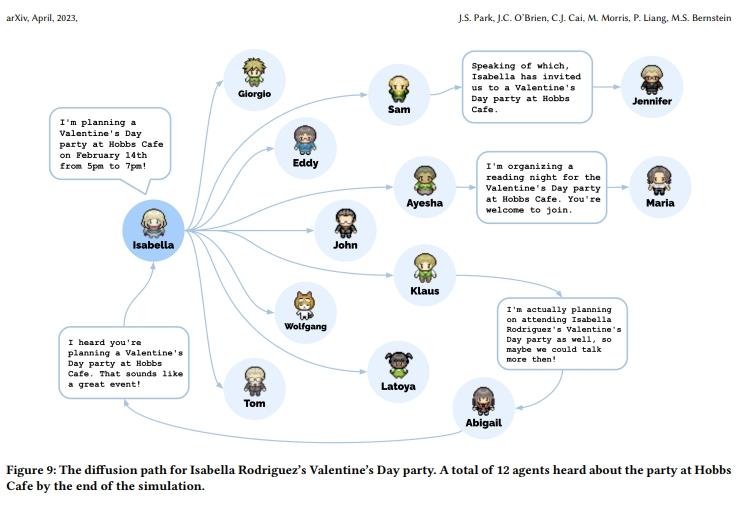
\includegraphics[width=0.8\textwidth]{birthdayParty.jpeg}
        %   \caption{Arch}
        %   \end{center}
        % \end{figure}

      \section*{Simulating Human Interaction}

        "Inworld Origins is a technical demo developed to demonstrate the power of generative AI-powered NPCs in video games. It showcases advanced NPC behavior and dialogue driven by artificial intelligence, leading to more immersive and personalized gaming experiences. The demo is set in a neo-noir sci-fi crime scene in the aftermath of an explosion in the city of Metropolis." source:google

          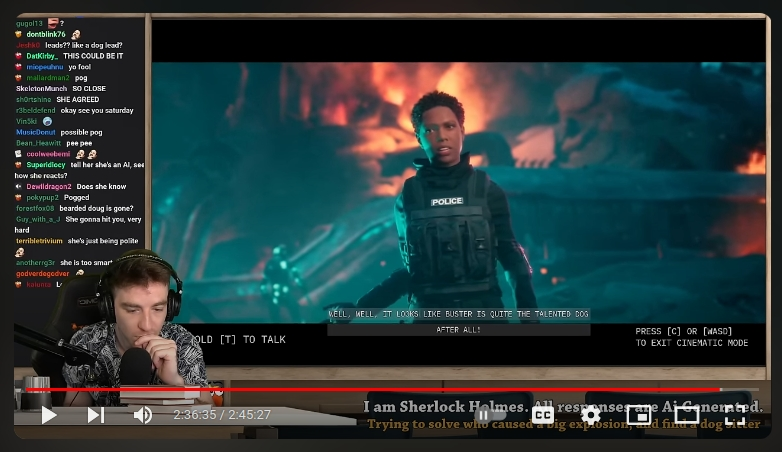
\includegraphics[width=0.8\textwidth]{dougdoug.jpeg}
          Screenshots of one demo using their openai abstraction layer.
          
        This team even offers multiple solutions for implementing such agents in popular environments such as Unreal.

        \textbf{Something that this project and the following one have in common is the presence of microphone input for live dialogue.}

          There is also a mod for the popular game Skyrim that allows the player to have fluid dialogue with any in-game character. 

        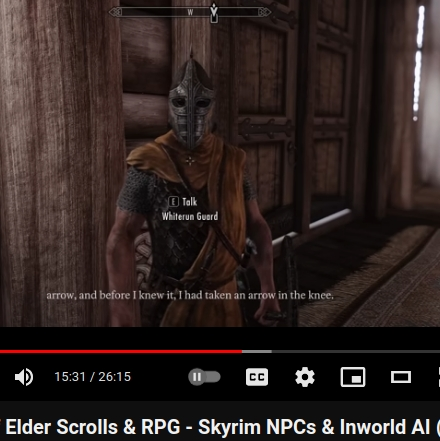
\includegraphics[width=0.8\textwidth]{arrow.jpeg}



          \subsection*{Ai interacting to Ai}
              One paper that i found beyond fascinating was Interactive Simulacra of Human Behavior.
        
              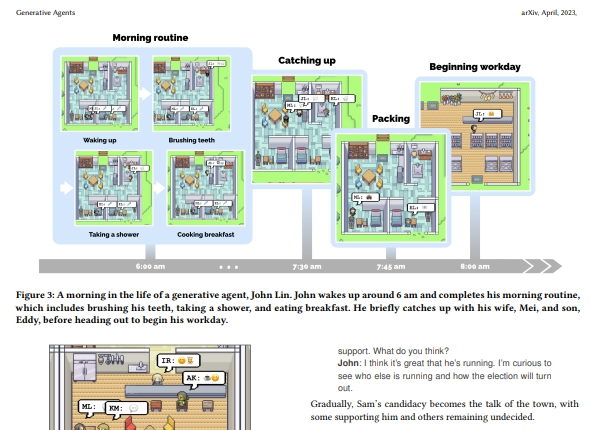
\includegraphics[width=0.4\textwidth]{morningRoutine.jpeg}
            
            They created an environment that allowed ml agents to communicate to one another. One of the most exciting outcomes was that one agent organised a birthday party and proceeded to invite other ml agents to the party. 

            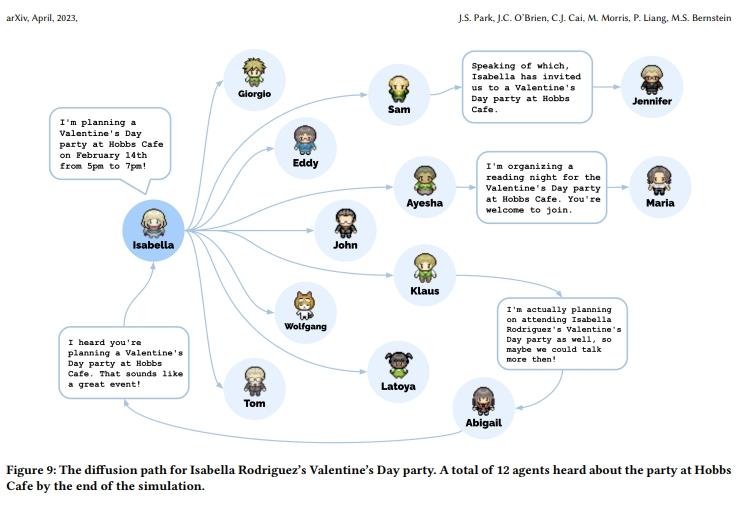
\includegraphics[width=0.8\textwidth]{birthdayParty.jpeg}

            The following goes more in detail over the implementatation design for one agent:
            
            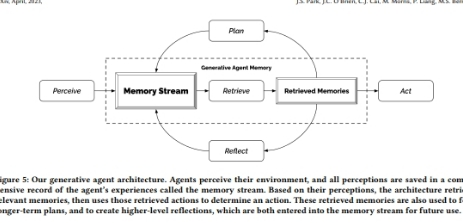
\includegraphics[width=0.8\textwidth]{DataStructure.jpeg}
            
            This design grants access to managing memories by long-time storage of relevant info. 

      
      \section*{Out-performing Human Performance}
        %   TODO: IMAGE 
        %   popular youtuber Code Bullet has a series where he "solves" games using AI models. He usually uses neural-networks for his solutions. 
          
          There are chess bots being developed that use machine learning in an attempt to "solve" the game of chess. So it is clear to say there is is a lot of incentivise towards acomodating machine learning algorithms into games.

        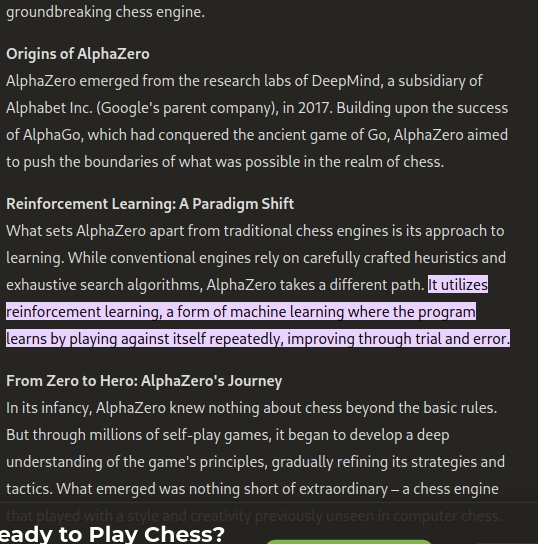
\includegraphics[width=0.8\textwidth]{alphazero.jpeg}
